\documentclass[12pt,twoside]{report}
\usepackage[left=2cm,top=3cm,right=2cm,bottom=3cm]{geometry}
\usepackage{fancyhdr}
\usepackage[danish]{babel}
\usepackage{lmodern}
\usepackage{pslatex} % Giver pænere font
\usepackage[utf8]{inputenc}
%\usepackage[T1]{fontenc}
\linespread{1.15} % linjeafstand
\setcounter{secnumdepth}{0}
\pagestyle{fancy}
\fancyhf{}
\fancyhead[LE,RO]{Gruppe A1}
\fancyhead[RE,LO]{Semesterprojekt}
\fancyfoot[LE,RO]{\thepage}
\usepackage{graphicx}
\graphicspath{ {img/} }


\begin{document}

\title{Semesterprojekt}
\date{29.\ maj, 2017}
\author{Tjalfe M\o ller, Kristian Krog, David Carl og Kasper Breindal}

\maketitle
\tableofcontents
\include{./tex/businesscase}
\include{./tex/Arkitektur}
\section{Brugergrænseflade og design}
Af Kasper\\\\
Vores mål med programmet var at skabe en nemt og velfungerende måde at designe en carport på.
Det skulle føles intuitivt, og ikke skabe forvirring når man arbejder i programmet.
Programmet har været igennem flere forskellige stadier, før det nåede frem til vores endelige løsning.
\\
\subsection{Gennemgang af grænseflade}
\subsubsection{For brugere}
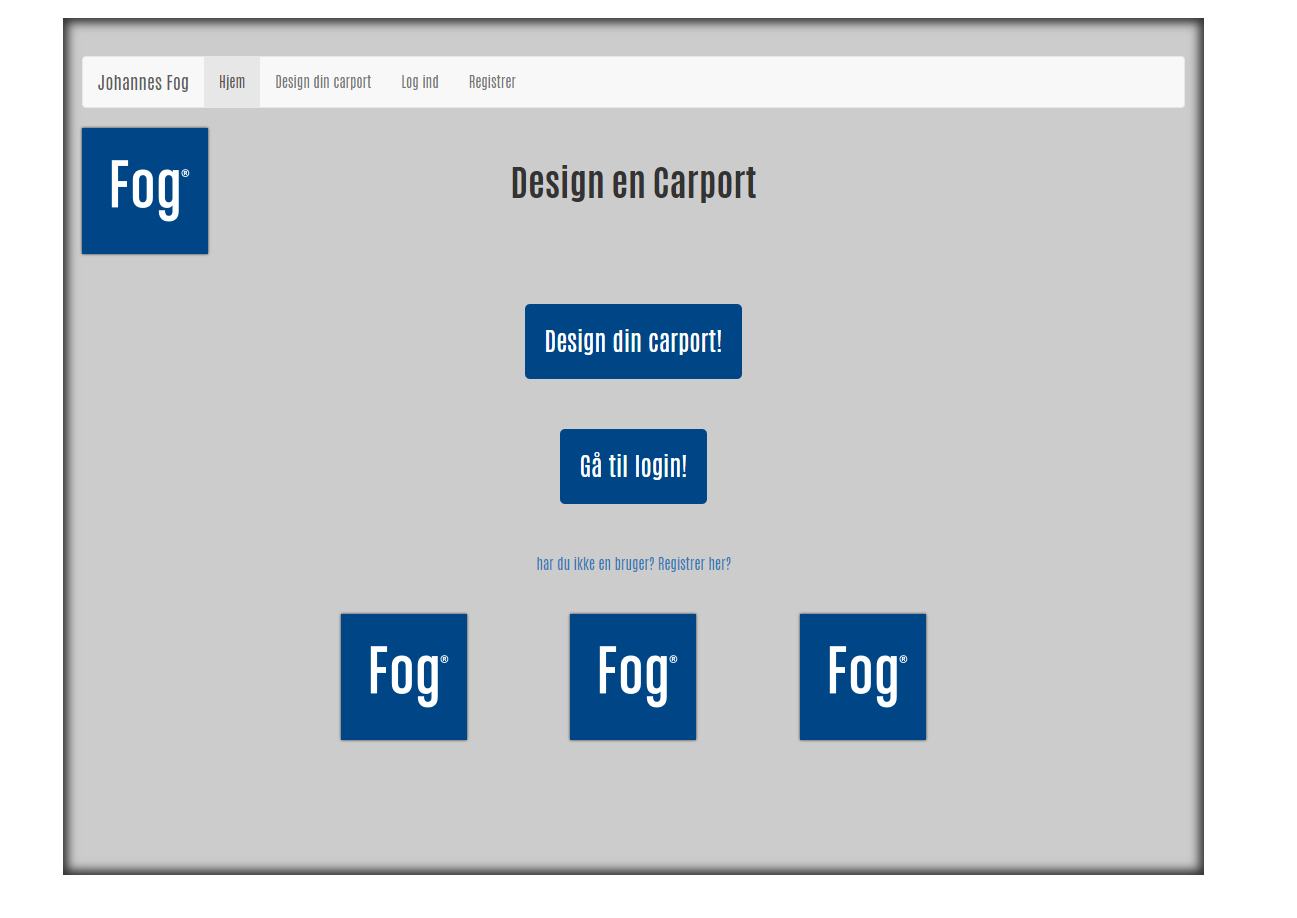
\includegraphics[width=\textwidth]{indexui}
Det første der skal tages stilling til for brugeren af siden er, om man vil logge in, registrere sig, eller bare prøve at designe sin carport.
Dette valg er bevidst stillet op for at tiltrække så mange potetientelle kunder som muligt.\\
Kunderne vil ikke som det første på siden oprette sig. Derfor får de muligheden for at arbejde med designværktøjet først, og gemme det senere.\\
Designmæssigt har vi ikke haft mulighed for at snakke med productowner Johannes Fog, og derfor har vi implementeret et design som er simpelt og nemt at finde rundt i.
Navigationsbaren i toppen kan bruges til at lede brugeren hen på den side de leder efter og har Johannes Fogs logo sat på.\\
\\\\
BILLEDE AF 3d
\\\\
Ved tryk på "design din carport"\ knappen ledes brugeren til vores 3D design program. Her kan brugeren køre sliders frem og tilbage, og vurdere hvordan deres carport skal se ud, og hvilke specifikke mål den skal have. Dette har den fordel at kunderne får en grafisk præsentation af hvordan deres carport kommer til at se ud, istedet for bare et billede af en tilfældig anden carport som firmaet engang. Når kunden føler at deres carport er som den skal være klikker de på "gem"\ knappen, og bliver herefter ledt videre til plantegningen af deres carport.
\\\\
BILLEDE AF 2D Her
\\\\
Her får kunden en 2D-plantegning af den carport de netop har designet i 3D-programmet. Tegningen har ikke alle mål sat på - dette er gemt til kunder der vælger at købe den carport de har designet. Samtidig med at tegningen er blevet genereret er carporten blevet gemt til brugeren, hvis man er logget ind. Hvis ikke, vil den bagefter bede dig om at logge in eller oprette dig.
\\\\
Billede af brugerpanel herefter
\\\\
Til slut kommer brugeren til brugerpanelet. Her kan de se den carport de har gemt, og kan trykke bestil, hvorefter ordren bliver sendt til databasen, til videre behandling af Fogs medarbejdere.

\subsubsection{for Fogs medarbejdere}
Fogs medarbejdere kan benytte dette samme system til behandling af ordrene. Hvis en medarbejder logger ind vil de blive taget til administratorpanelet. Her kan

\subsection{Tekniske detajler}
Websiderne i projektet er skrevet i JSP, CSS og JavaScript, og benytter sig af JSTL og eksterne libraries så som THREE.js, jQuery og Bootstrap til at forbedre udseendet af projektet og gøre projeket kompatibelt med flere forskellige browsere og styresystemer. Så vidt muligt bliver disse libraries hentet eksternt, via et Content-Delivery Network (CDN). Dette skaber den fordel at brugerne kan have disse pakker cached fra tidligere brug på andre websider i forvejen, og derfor ikke behøver at hente dem igen. Det betyder også at pakkerne ikke kommer til at ligge på firmaets server, og derfor kan lette datatrafikken på serveren, og derved køre mere stabilt.\\
Workflowet er udarbejdet efter at kunne indsættes i et hvert webside-design, og til at kunne omskrives til andre programmeringssprog.\\
Dette giver os som gruppe muligheden for at udvikle i det sprog vi kender til (Java), samtidig med at det kan omskrives til, for eksempel, en C\# og ASP.Net baseret kodebase, hvilket er meget udbredt i Danmark.
\section{SQL Queries}
Af Kasper\\\\
Alle metoder til at behandle SQL statements til vore MySQL database findes i DataAccessObject-klassen. Vi benytter os af PreparedStatements for at gøre systemet hurtigere og mere stabilt, og for at sikre os mod SQL-injection angreb.\\
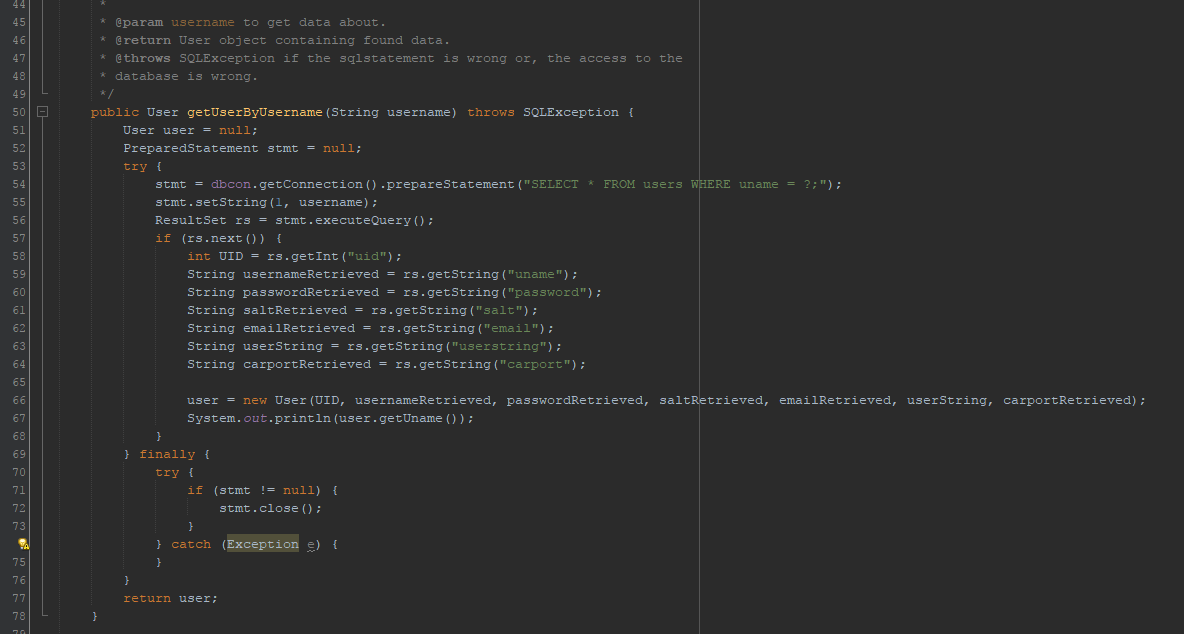
\includegraphics[width=\textwidth]{sqlstatement}

\include{./tex/features}
\section{Testing}
Af Kasper\\\\

I softwareudvikling er det vigtigt at sikre sig, at det der bliver produceret også fungerer som det skal. Firmaer benytter software til både behandling af persondata, lønstyring og behandling af anden fortrolig data, og derfor er det vigtigt, at alt er sikkert og fungere efter hensigten når det bliver sendt live.

\subsection{Manuel Testing}
Vi har alle i gruppen individuelt gået igennem alle funktioner i programmet, og sikret os at det hele fungerer. Dette har inkluderet at prøve at sende forkert data i input-felter, se sider, hvor man skal være logget ind som adminstrator, uden at være det og tjekke efter ødelagte links. Vi har derefter fikset alle fejl der blev fundet, for at levere et bedre produkt.\\
\subsection{Automatiseret Testing (JUnit)}
Vi har Unit Tests på de mest essentielle metoder i klassen DataAccessObject, da dette er den klasse der foretager de fleste vigtige metodekald.
\include{./tex/errors}
\include{./tex/futureimplementations}
\section{Arbejdsmetoder}
Af Kasper\\\\
En del af opgaven var at følge Scrum og Agile principper til at få fremstillet projektet. Gruppen tog dette nogenlunde til sig, dog krævede det en tilvænningsperiode i starten af samarbejdet før alle var med på hvordan dette skulle udføres.\\
Vi har været 4 mand i gruppen, og selvom Scrum bygger på grupper af 6-8 mand, har dette har været en meget passende størrelse i forhold til uddellegering af opgaver, og så er man ikke for mange til møderne, som derfor bliver overkommelig længde.
Derudover gør det mindre antal gruppemedlemmer også det, at det ofte er nemmere at komme til enighed i diskussioner, men at alles stemme bliver hørt, da hver mand jo tæller for 25\%.\\
Vi har i vores gruppe aftalt at vi de fleste dage mødtes på skolen for at arbejde, for at sikre os at alle får foretaget det de skal, og det på den måde bliver nemmere at hjælpe hinanden med problemer man måtte møde undervejs.

\subsection{Værktøjer}
Til versionsstyring har vi benyttet os af Git og GitHub. Dette har fungeret til al tilfredsstillelse, og vi har sjældent haft merge conflicts. Gruppen har sigtet efter at arbejde efter feature-branching, altså at hver ny tilføjelse laves i sin egen branch, og derefter merges ind i master til det fungerende projekt.\\\\
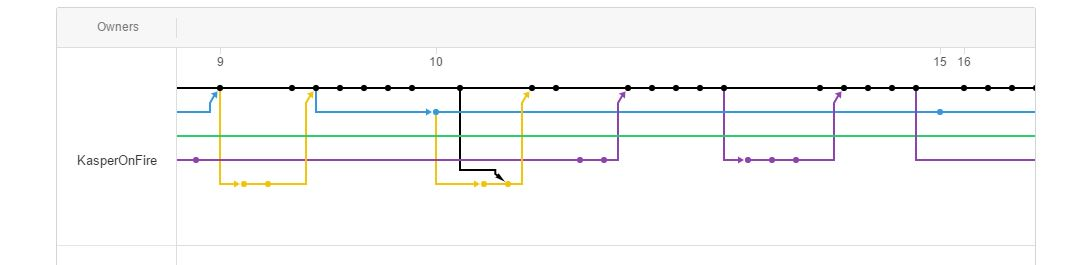
\includegraphics[width=\textwidth]{branches}\\\\


\subsection{Scrum}

\subsection{Agile development}
\include{./tex/conclusion}



\end{document}